%%%%%%%%%%%%%%%%%%%%%%%%%%%%%%%%%%%%%%%%%%%%%%%%%%%%%%%%%%%%%%%%%%%%%%%
%%%%  Load the document class and packages                         %%%%
%%%%%%%%%%%%%%%%%%%%%%%%%%%%%%%%%%%%%%%%%%%%%%%%%%%%%%%%%%%%%%%%%%%%%%%
\documentclass[a4paper]{report}
\usepackage{epsfig} %to insert PostScript figures
\graphicspath{ 
  {scanningFigs/} 
}

%Change figure names
\renewcommand{\figurename}{Fig}

\usepackage[bf,footnotesize]{caption} % make captions small and label bold
\usepackage{graphicx}


\addtocounter{chapter}{1} %Because starting at zero is silly
\makeatletter
\renewcommand{\thesection}{\@arabic\c@section}
\renewcommand{\thefigure}{\@arabic\c@figure}
\makeatother

\usepackage[a4paper,margin=2.7cm,tmargin=2.5cm,bmargin=2.5cm]{geometry} 
\usepackage{textcomp}  %To make nice degree symbols and others\usepackage[bf,footnotesize]{caption} % make captions small and label bold
\usepackage{wrapfig}





\begin{document}




%set the number of sectioning levels 
\setcounter{secnumdepth}{2}

\begin{center}
\textbf{\Large{Scanning Software \& Data Acquisition}}
\end{center}

\section{Introduction}

In widefield microscopy the entire field of view is illuminated and a great deal of scattered light from outside of the focal plane ends up in the image plane. 
These scattered photons create blur and reduce contrast since they fail to satisfy the image-forming condition, arriving at the image plane at a location \textit{not conjugate} with their origin.
Fluorescence-based scanning microscopy can greatly mitigate the problem of scattering. 
A laser beam is scanned across the sample where it excites fluorophore molecules. 
Emitted fluorescence is collected via the objective and detected at a photomultiplier tube (PMT). 
No image is formed on the PMT (it's a `single pixel'), instead the image is constructed \textit{post-hoc} on a computer with the spatial origin of the emitted fluorescence determined by the position of the laser beam in time.
In confocal microscopy, emitted fluorescence arising away from the focal point is rejected by a pinhole conjugate with the sample and near the PMT. 
With 2-photon microscopy, the excitation spot is highly restricted so the origin of all collected photons is known (Fig.~\ref{1pvs2p}). 

\begin{figure}[h]
\centering
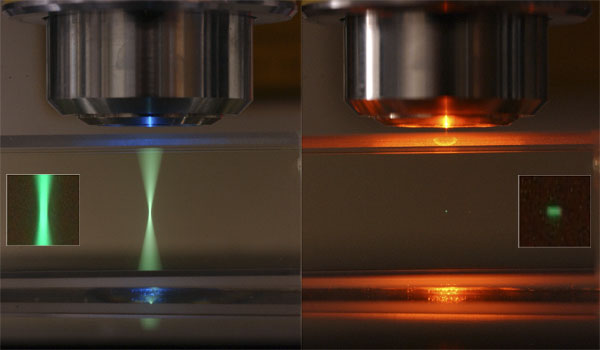
\includegraphics[width=4.5in]{1Pvs2PFluorescence.png}
\caption{A blue (488nm) laser of the sort used in confocal imaging excites an entire column of sample leading to green fluorescence (left).
A pulsed IR laser excites only at the focal point, as this is the only location where the density of photons is great enough for the 2-photon effect to take place.}
\label{1pvs2p}
\end{figure}



\subsection{Goals}
In the following exercises you will learn how to write simple scanning software using MATLAB and NI DAQmx in order to run a transmitted light laser scanning microscope. 
The goals of today are:
\begin{itemize}
\setlength\itemsep{0.15em}
\item Learn how to drive the scan mirrors using analog output waveforms from a data acquisition card. 
\item Understand how an image is built on a computer screen from a photodiode signal. 
\item Become familiar with the basics of controlling National Instruments data acquisition hardware.
\item Understand how a beam expander is used to conjugate scanning mirrors onto the objective back aperture to image microscopic samples.
\end{itemize}

\clearpage


\section{Driving the scan mirrors}
A scanning microscope has two scan mirrors (`galvos'): one for $x$ and one for $y$ motion.
Each galvo is connected to a driver card that both powers it and controls the mirror position angle (Fig.~\ref{scanners}). 


\begin{figure}[h]
\centering
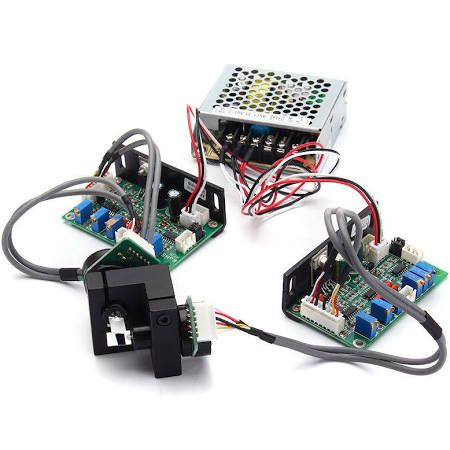
\includegraphics[width=2.25in]{scanners.png}
\caption{A pair of scan mirrors mounted orthogonally to each other and each connected to control card. The two control cards share a power supply.}
\label{scanners}
\end{figure}

Set up the rail as shown in Fig.~\ref{scannersOnRail}.
The scanners are bolted to the rail via the LCP11/M.
The rail carriage with the iris should be able to freely slide up and down the length of the whole rail.
The scanners need to be powered and receive a 0~V command signal. 
A TA will show you how to do this. 

\begin{figure}[h]
\centering
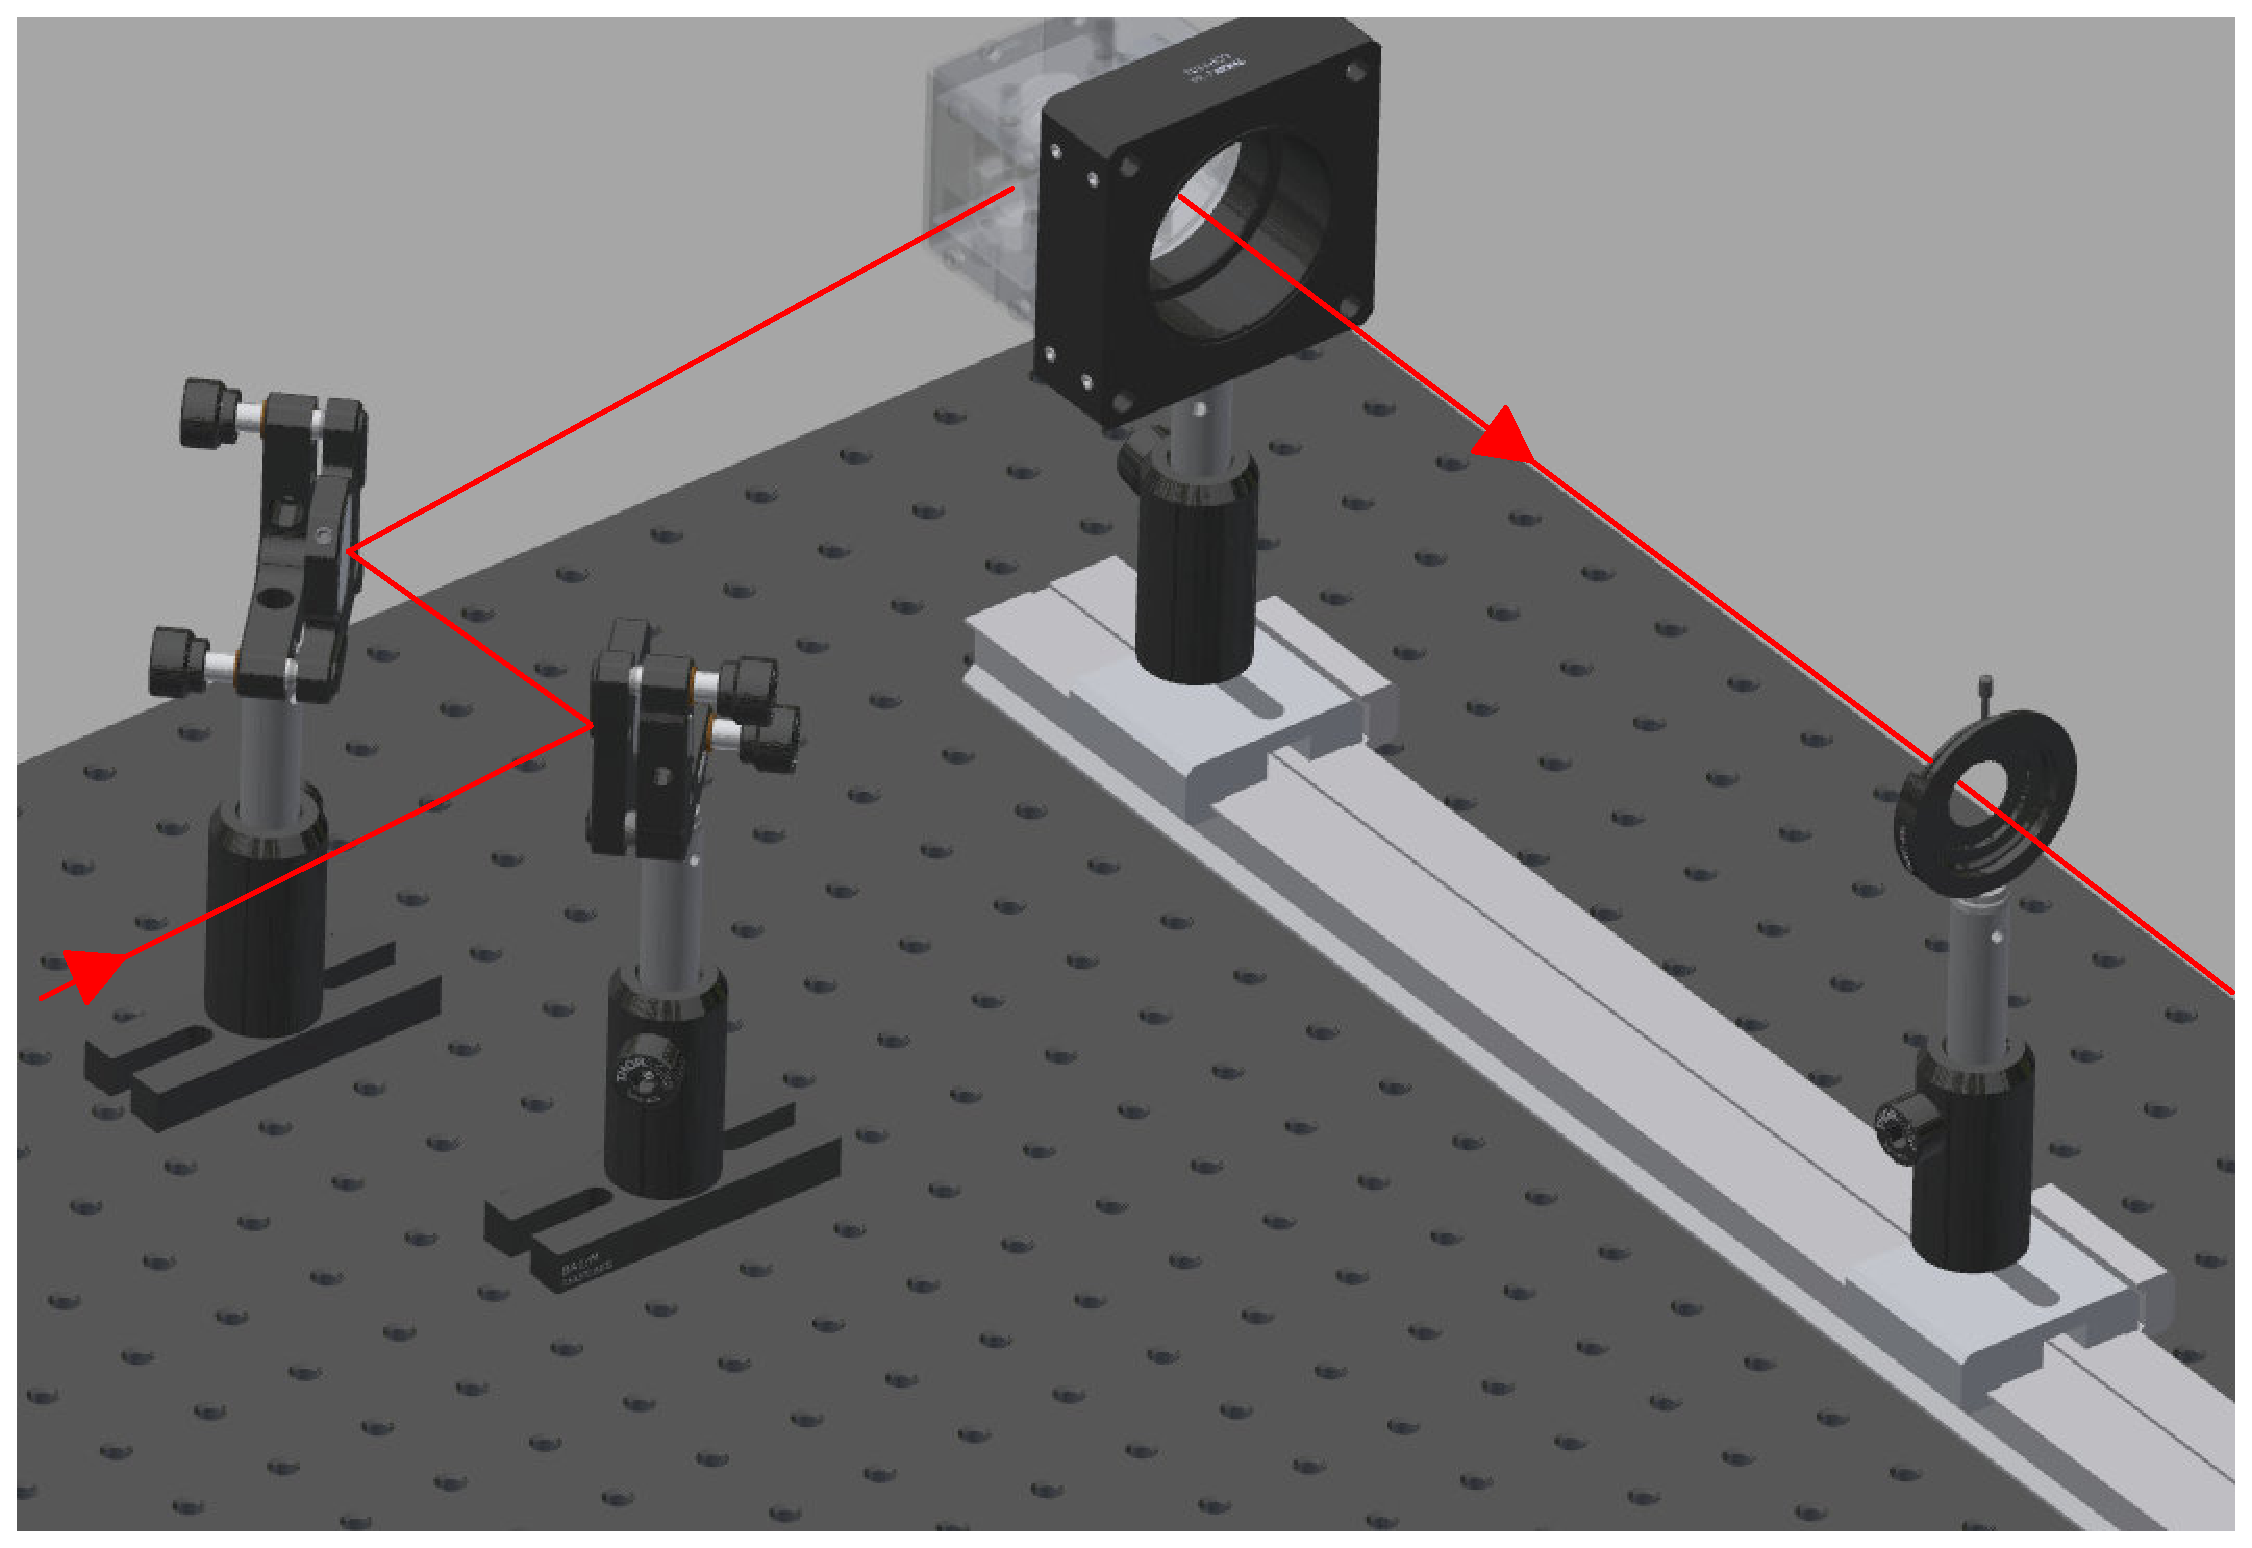
\includegraphics[width=3.0in]{InitialScannerSetup.eps}
\caption{The scanners mounted to the rail along with an iris. 
The two mirrors will route the beam into the scanner box.}
\label{scannersOnRail}
\end{figure}

\noindent
Direct the laser beam using two adjustable mirrors such that it hits the middle of the scan mirrors then comes out at 90 degrees with respect to the incoming beam (as shown in Fig.~\ref{scannersOnRail}). 
Using the iris as a target, ensure the beam runs straight down the rail. 
Move the scanners or even the rail if you need to.
It's OK for our purposes if the alignment isn't \textit{perfect}: a couple of beam diameters is adequate. 
Tips:
\begin{itemize}
\setlength\itemsep{0.15em}
\item Place one routing mirror close to the scanners and the other some distance away. 
\item Have all mirrors roughly square with respect to each other before starting.
\item Use adjustment screws for fine-alignment only.
\end{itemize}


\clearpage

\subsection{Controlling the scan mirrors}

\begin{itemize}
    \item Open NI MAX (Measurement \& Automation Explorer),
        \begin{enumerate}
            \setlength\itemsep{0.15em}
            \item Select the DAQ device from the list on the left then hit `Test Panels'. 
            \item Select the `Analog Output' tab (Fig.~\ref{DAQMX}).
            \item Set `Mode' to `Voltage Sinewave Generation' and set the amplitude to about `5V'.
            \item Leave the `Rate' at `1000'. This will produce a 1~Hz sine wave.
            \item Connect the analog outputs to the osciloscope and confirm you get waveforms out of both channels. 
        \end{enumerate}

    \item Turn on the laser, copy signals to the scanner controller analog inputs and try driving the scan mirrors with the 1~Hz signal.  
    \item Set `Rate' to `50,000' to produce a 50~Hz motion. What does the outgoing beam look like now?
    \item Now try the `DC' option under `Mode' and explore what happens when you apply a variety of constant non-zero voltages (press `Update' to apply your chosen voltage to the device).
\end{itemize}


\begin{figure}[h]
\centering
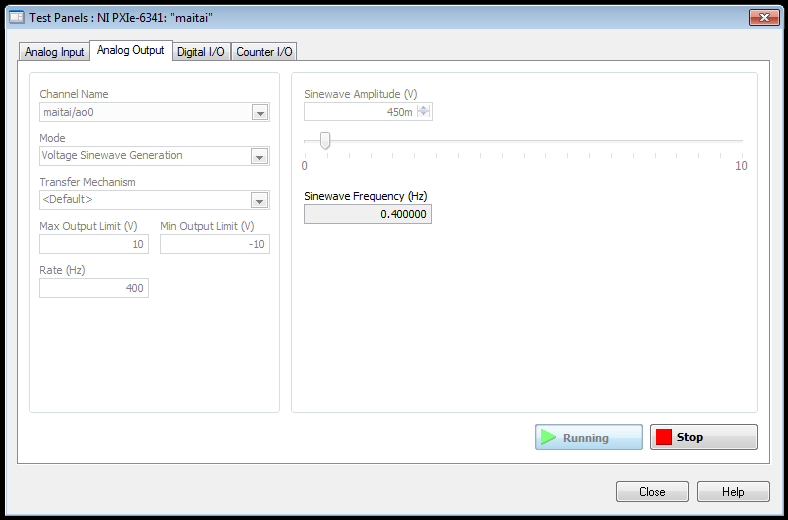
\includegraphics[width=3.5in]{MAX_for_1D.png}
\caption{The NI MAX test panel for analog output.}
\label{DAQMX}
\end{figure}



\clearpage

\section{Building the scan pattern}

You will now use MATLAB to generate scan waveforms and explore how to build an effective 2-D scan pattern. 
Before starting, make the following modifications to the DAQ breakout box. 

\begin{itemize}
    \setlength\itemsep{0.15em}
    \item Copy \texttt{AO0} to \texttt{AI0} with a BNC cable. will allow us to acquire and monitor the $x$ galvo command signal.
    \item Connect \texttt{AI1} to the galvo position output lead. This will allow us to compare the actual mirror position with the command position.
\end{itemize}

\noindent
You will now use a MATLAB class called `wavformTester' to explore different scanning waveforms.
The class is part of the SimpleMScanner\footnote{\textit{https://github.com/tenss/SimpleMScanner}} repository, which contains basic scanning software written in MATLAB.


\begin{itemize}
\setlength\itemsep{0.15em}
\item In MATLAB, run \texttt{edit waveformTester.m} to bring up the code. 
\item Run \texttt{S=waveformTester;}, which will send a sinusoidal command signal to the scanner and create an object called \texttt{S} in the base workspace.
\item At any time you can stop acquisition and disconnect from the DAQ by closing the figure window.
\end{itemize}

\noindent
With the default scan settings you should see something similar to that shown in Fig.~\ref{waveformTester01}.
You will see a red sinusoid, which is the galvo position feedback signal. 
Underneath the red trace is a black trace that represents the command signal. 
The inset blue sub-plot shows the position signal as a function of the command signal. 
The frequency of the waveform is displayed in both the window title and at the command line. 


\begin{figure}[h]
\centering
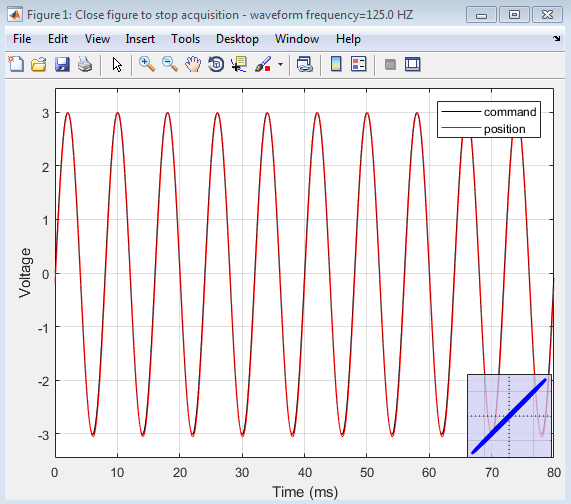
\includegraphics[width=2.5in]{waveformTester01.png}
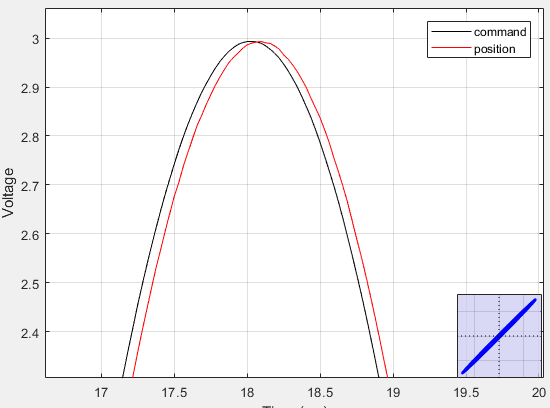
\includegraphics[width=2.08in]{waveformTester01_zoom.png}
\caption{Left: \texttt{waveformTester} running with default settings. 
        The waveform frequency is shown in the figure title bar. 
        The galvo command signal is shown in black and the feedback signal from the galvo control box is shown in red. 
        The inset blue plot shows the feedback signal as a function of the command signal.
         Right: A zoomed-in view showing the close correspondence between the command signal (black) and the actual galvo position (red).
         When zoomed-in you will notice the plot is regularly updating.}
\label{waveformTester01}
\end{figure}


\noindent
Read through the code and satisfy yourself that you understand how it works. 
Pay particular attention to how the waveform is built. 

\begin{itemize}
    \setlength\itemsep{0.15em}
    \item The waveform amplitude is scaled by the \texttt{galvoAmp} property.
    \item For the current sine wave, \texttt{pixelsPerLine} is the number samples in one cycle. 
    \item The waveform is repeated \texttt{numReps} times, and this many cycles are plotted at once. 
    \item The \texttt{generateScanWaveform} method builds the waveform, which may be either a sawtooth or a sine wave according to the value of \texttt{waveformType}.
\end{itemize}


\clearpage
\subsection{The effect of command signal frequency}
The scanners have inertia so their ability to follow the command waveform will depend upon its shape and frequency. 
Let's try changing the frequency. 

\begin{itemize}
\item Close the figure window (take a screenshot first if you want to compare before and after) and edit the \texttt{sampleRate} property.
Increase it from the default 32E3 to 128E3 (meaning $128~kS/s$). 
\texttt{sampleRate} is used by the \texttt{ratecfgSampClkTiming} methods of the AI and AO DAQmx tasks to set the sample rate.
This is done in the \texttt{connectToDAQandSetUpChannels} method of \texttt{waveformTester}.
\item Re-start the \texttt{waveformTester} object (close window and run command again). 
\item Notice the larger phase lag between the position and command and how this is reflected in the blue X/Y plot. 
\end{itemize}

\noindent
Now try using fewer samples per cycle, which is the other way of increasing the mirror frequency. 
Close the figure window, set \texttt{pixelsPerLine} from the default 256 to 128, and restart.
At 128 \texttt{samplesPerLine} and $128~kS/s$ sample rate the scanner runs at $1~kHz$.

\subsection{Different waveform types}
Return the sample rate to 32E3 and the number of samples per line to 512. 
Change the \texttt{waveformType} property from `sine' to `sawtooth' and restart the \texttt{waveformTester}. 
How well is the scanner following the command waveform? 
Satisfy yourself that you understand why the blue inset plot looks as it does. 
What are the advantages and disadvantages of this new waveform for building 1-D images?
Hint: think about how the beam changes speed during the sawtooth in comparison to the sinewave.
Think also how you might build the image on the PC and how well the mirrors follow the sawtooth waveform.


\clearpage

\section{Building scan waveforms}

So far you have moved only the $x$ mirror and considered 1-D images. 
Obviously you need to move both mirrors at the same time to get a 2-D scan pattern and image full frames.
Before proceeding, let's get both mirrors moving at the same time. 
First of all, re-wire your setup so that the two analog outputs are copied to channels 1 and 2 of the oscilloscope.
Now run the command \texttt{vidrio.AO.hardwareContinuousVoltageNoRegen\_2chans} to play out two sine waves.
Satisfy yourself that your understand why the beam motion looks the way it does based upon the oscilloscope traces.


\subsection{Acquiring a 2-D image}

In this section you will modify \texttt{waveformTester.m} in order to turn it into a simple piece of scanning software.
Since we will be making an image with the photodiode signal, connect the photodiode to \texttt{AI0} using a BNC cable.
You will need to produce suitable $x$ and $y$ waveforms and also to plot the photodiode signal as an image. 
Use \texttt{vidrio.AO.hardwareContinuousVoltageNoRegen\_2chans} to figure out how to add the second analog output channel.
Aim for waveforms that will produce square images at about 0.5 frames per second. 
Start off with a sample rate of 32E3 and change the frame rate by altering the image size.
Hints:
\begin{itemize}
    \setlength\itemsep{0.15em}
    \item The waveforms are stored in an N-by-2 array, where each row is a different time point. You only need to modify code in the \texttt{generateScanWaveform} method.
    \item Modify \texttt{obj.hAOTask.createAOVoltageChan} to use both channels 0 and 1.
    \item The \texttt{numReps} property can be used to set the number of scan lines per frame.
\end{itemize}

\noindent

Once you have the waveforms looking reasonable judging by the oscilloscope and the scan pattern, it's time to modify the code to handle the photodiode signal. 
To begin with, let's just ensure we can display the incoming photodide signal as a line plot.

\begin{itemize}
    \setlength\itemsep{0.15em}
    \item Modify \texttt{obj.hAITask.createAIVoltageChan} to acquire only on \texttt{AI0}.
    \item In the constructor you can remove the code for making the blue inset plot and remove the line which creates \texttt{obj.hPltDataAO1}, as we won't be plotting that channel.
    \item Modify the \texttt{readAndDisplayScanData} method to update only \texttt{obj.hPltDataAO0}. Remove lines relating to the other plots. 
    \item Allow the beam to scan over the photodiode and test the code. 
    You should see something like that shown in Fig.~\ref{lineOnPD}. 
\end{itemize}

\noindent


\begin{figure}[h]
\centering
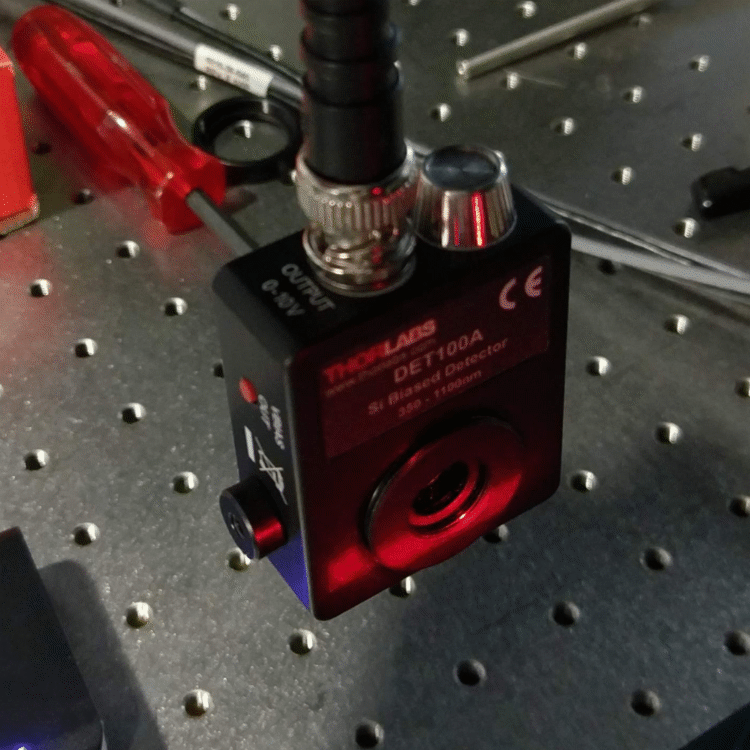
\includegraphics[width=1.8in]{BeamScanningOverPhotoDiode.png}
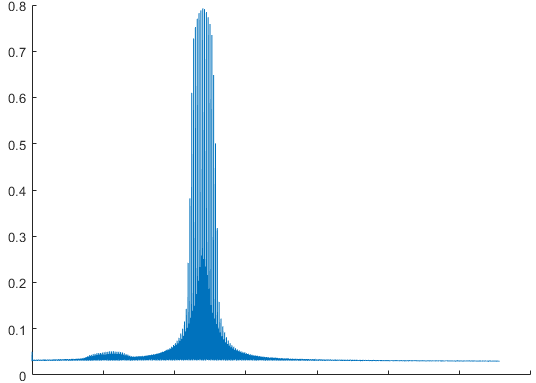
\includegraphics[width=2.4in]{photodiode_lineTrace.png}
\caption{Left: The beam scanning over the photodiode
         Right: The photodiode signal plotted on screen as a time trace.
         The this plot was obtained by positioning the photodiode about 30 cm from the scanners and using a waveform amplitude of about 4~V. 
         Under these circumstances the beam is only scanning over the photodiode for a short period of time, producing the peak you see in the plot. }
\label{lineOnPD}
\end{figure}

\noindent
Once you have reached the stage above, you know that you're pulling in the data correctly and all you need to do is reshape them into an image instead of a line plot.
Hints:
\begin{itemize}
    \setlength\itemsep{0.15em}
    \item In the constructor, the line \texttt{obj.hPltDataAO0 = plot(obj.hAxes, zeros(100,1), '-k');} should instead create a blank image using \texttt{imagesc}. Any size is fine.
    \item In the \texttt{readAndDisplayData} method you will need to modify the plot object's \texttt{CData} property instead of the \texttt{YData} property. 
    \item You already know what size to \texttt{reshape} the data too, since you know the number scan lines and the number of lines per frame.
    \item Minor changes, like altering the color-scale look-up table, can be made whilst the code is running.
\end{itemize}

\noindent
Place the photodiode around 30~cm from the scanners and use and amplitude of 2 or 3~V.
Fire up the code and try to get an image. 
What do you see?
Is it what you expect? Hint: think about how the image is being assembled and how well the scanner follows the command signal.
What happens if you slide the photodiode up and down in the post holder?
Now move the photodiode closer to the scanners and use a scan pattern that only just fills the photodiode active area. 
Note how the image changes. 
Stick a small paper square to a coverslip and place it over the photodiode active area and watch the image.
You might get better results by focusing the beam onto the photodiode with an $f=60~mm$ lens. 

\begin{figure}[h]
\centering
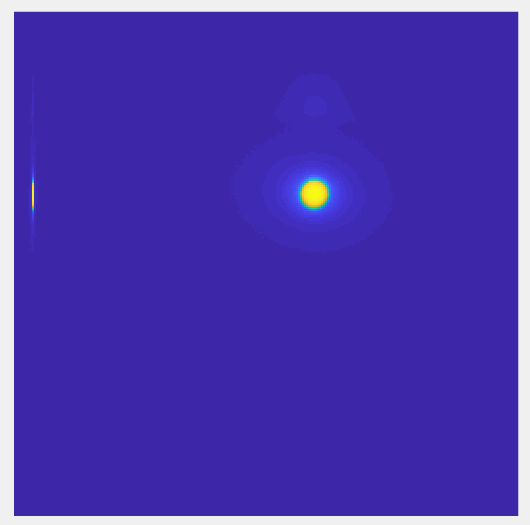
\includegraphics[width=2in]{distantPhotoDiode.png}
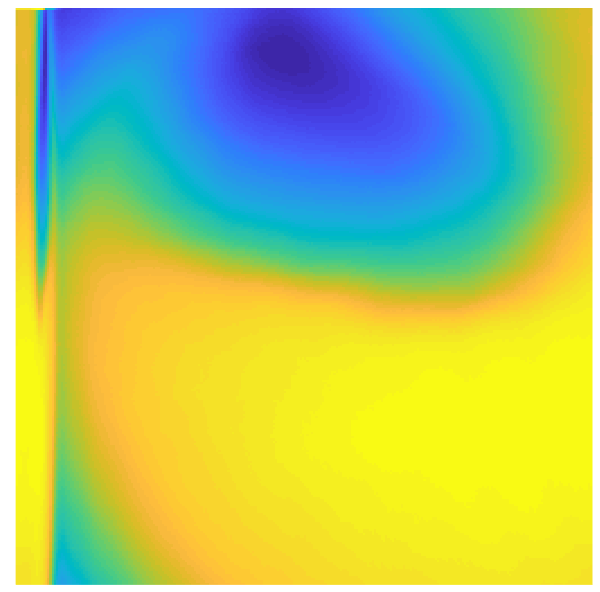
\includegraphics[width=2in]{PhotoDiode_2Dimage.png}
\caption{Left: With a large-angle scan pattern and the photodiode far from the scanners you end up with an image of the whole scan-field showing the position of the photodiode within the scan-field.
         Right: Here the scan angle is reduced to just fill the photodiode and a small piece of tape is placed on the middle of a coverslip in front of the photodiode. 
         An image of the tape piece is then be formed on the computer.}
\label{PDimage}
\end{figure}



\clearpage


\section{Obtain an image of a microscopic sample}
You will now use a microscope objective to scan the beam over a sample and obtain an image. 
You already have the scanners on the end of an optical rail with the beam aligned to the rail. 
With a help of a TA you will add a scan lens, tube lens, and 4x objective to form a simple scanning microscope. 
the scan lens and tube lens serve two purposes:

\begin{enumerate}
\setlength\itemsep{0.1em}
\item They placed the scanners in a conjugate plane to the back aperture of the objective. 
\item They form a beam expander which allows the beam to fill the back aperture of the objective.
\end{enumerate}

\noindent
Once everything is set up, play your scan pattern and use a card to observe the beam motion through the optical system. 
What do you see at $1f$ from the scan lens?
What do you see at the working distance of the objective?
What do you see at the objective back aperture?
Satisfy yourself that all those things make sense.

\noindent
Place a slide containing an EM grid at the working distance of the objective. 
Place a photodiode close to the back of the slide and hook it up to \texttt{AI0} on your DAQ. 
You may get a better image with a collection lens in front of the detector, but this isn't critical\footnote{Or even K\"{o}hler, for that matter.}.
Focus the beam onto the grid as best you can by eye.
Now it's time to get an image!


\section{Advanced Topics}
If you have completed the above and still have time, you can explore any of the following topics which take your fancy.



\subsection{Trying different waveforms in ScanImage}
The sawtooth waveform is commonly called a `unidirectional scan waveform' because we acquire data in one direction only (the slow ramp). 
It's easy to build an image from this waveform but a lot of time is wasted during the $x$ mirror flyback. 
You could optimize this by using both the outward and return portions of the waveform to build an image. 
Think how would you change your sawtooth waveform to allow for this `bidirectional' scanning? 

ScanImage supports both unidirectional and bidirectional scanning. 
Start it by typing `scanimage` into the command line and set it up with the help of a TA. 
`Focus` starts scanning and `Configuration` window allows you to change scan settings. 
Get an image of the photodiode and explore how this alters when you change the scan settings. 
Try to get a nice image of the photodiode without artifacts using bidirectional scanning. 


\subsection{Correcting image artifacts}
We built images based on the command waveforms. 
In other words, we assume the beam is located where we asked it to be and we placed the pixels at that location.
Since the actual beam position does not follow the expected position, this produces artifacts. 
Try to come up with a way of correcting the image. 
Perhaps you could use the mirror feedback signal, or use the command signal but remove the non-linear portions, or some mixture of those options. 

\end{document}
